%——————————————————————————————————————————————————
\documentclass[sigconf,twocolumn,nonacm=true]{acmart}
\usepackage[utf8]{inputenc}
\setlength{\parindent}{0pt}
\setlength{\parskip}{6pt plus 2pt minus 2pt}
\newcommand{\tighten}{\vspace*{-6pt plus -2pt minus -2pt}} %Can be used to remove unwanted ¶ spacing before/after figures, align blocks, etc.

%——————————————————————————————————————————————————
%JPH Packages & Commands
\usepackage{multicol,multirow,mathtools,centernot,mathrsfs,pifont,amssymb,algorithm2e,adjustbox,graphicx}
\newcommand{\cmark}{~\text{\ding{51}}~} %checkmark
\newcommand{\xmark}{~\text{\ding{55}}~} %x-mark
\newcommand{\smark}{~\text{\ding{78}}~} %star
\newcommand{\emd}{\text{\textemdash}} %shorter em-dash (—) command
\let\thorn\th %goodbye
\renewcommand\th{^{\text{th}}} % 5^th, etc
\newcommand{\st}{^{\text{st}}} % 1^st, etc
\newcommand{\rd}{^{\text{rd}}} % 3^rd, etc
\newcommand{\inv}{^{-1}} %g^-1, etc
\newcommand{\e}[1]{\times10^{#1}} %scientific notation
\newcommand{\rf}[1]{^{\overline{#1}}} %rising factorial
\newcommand{\ff}[1]{^{\underline{#1}}} %falling factorial
\newcommand{\ch}[2]{\ds{#1 \choose #2}} %shorter/simpler syntax for choose
\newcommand{\chf}[2]{\ds\frac{#1 !}{#2 ! \enc{#1 - #2}!}} %converts choose to fraction form
\newcommand{\enc}[1]{\left( #1 \right)} %enclosed by scaling ()
\newcommand{\encl}[1]{\left[ #1 \right]} %enclosed by scaling []
\newcommand{\embrace}[1]{\left\lbrace #1 \right\rbrace} %enclosed by scaling {}
\newcommand{\vect}[1]{\left\langle #1 \right\rangle} %enclosed by scaling <>
\newcommand{\vvec}[1]{\vec{\boldsymbol{#1}}} %vector variable formatting
\newcommand{\abs}[1]{\left\lvert #1 \right\rvert} %enclosed by scaling | bars
\newcommand{\ceil}[1]{\left\lceil #1 \right\rceil}  %enclosed by scaling ceil bars
\newcommand{\floor}[1]{\left\lfloor #1 \right\rfloor} %enclosed by scaling floor bars
\newcommand{\norm}[1]{\lVert #1 \rVert} %enclosed by (non-scaling) double-| bars
\newcommand{\norml}[1]{\left\lVert #1 \right\rVert} %enclosed by 'large' (scaling) double-| bars
\newcommand{\err}{\mathcal{E}} %curly E for error
\newcommand{\bigo}[1]{\mathscr{O}\enc{#1}} %curly O for big-O order
\newcommand{\eps}{\epsilon} %shortcut for epsilon
\newcommand{\N}{\mathbb{N}} %naturals
\newcommand{\Z}{\mathbb{Z}} %integers
\newcommand{\Q}{\mathbb{Q}} %rationals
\newcommand{\R}{\mathbb{R}} %reals
\newcommand{\C}{\mathbb{C}} %complex
\newcommand{\G}{\mathcal{G}} %group
\newcommand{\s}{\mathcal{S}} %set
\newcommand{\powset}[1]{\mathscr{P}\enc{#1}} %curly P for power set function
\newcommand{\ran}[1]{\mathscr{R}\text{an}\enc{#1}} %range function
\newcommand{\dom}[1]{\mathscr{D}\text{om}\enc{#1}} %domain function
\newcommand{\kernel}[1]{\mathcal{K}\text{er}\enc{#1}} %fancy kernel function
\newcommand{\glnr}[1][n]{GL_{#1}\enc{\R}} 
\newcommand{\slnr}[1][n]{SL_{#1}\enc{\R}}
\newcommand{\ds}{\displaystyle} %shortcut for displaystyle
\newcommand{\lump}[1]{\mathclap{\substack{#1}}} %allows multiple lines to be stacked where they normally can't, without affecting box width
\newcommand{\Integral}[2]{\ds\int_{\lump{#1}}^{\lump{#2}}} %shorter syntax with formatting upgrades
\newcommand{\Sum}[2]{\ds\sum_{\lump{#1}}^{\lump{#2}}} %shorter syntax with formatting upgrades
\newcommand{\Prod}[2]{\ds\prod_{\lump{#1}}^{\lump{#2}}} %shorter syntax with formatting upgrades
\newcommand{\Union}[2]{\ds\bigcup_{\lump{#1}}^{\lump{#2}}} %indexed union
\newcommand{\Intersect}[2]{\ds\bigcap_{\lump{#1}}^{\lump{#2}}} %indexed intersection
\newcommand{\edp}[2]{\ds\bigoplus_{\lump{#1}}^{\lump{#2}}} %indexed external direct product
\newcommand{\Lim}[2]{\ds\lim_{\lump{\substack{#1} \to \substack{#2}}}} %shorter syntax with formatting upgrades
\newcommand{\Min}[1]{\ds\min_{\lump{#1}}} %shorter syntax with formatting upgrades
\newcommand{\Max}[1]{\ds\max_{\lump{#1}}} %shorter syntax with formatting upgrades
\newcommand{\eval}[2]{\bigg\mid_{\lump{#1}}^{\lump{#2}}} %evaluation bar
\newcommand{\evall}[2]{\Big\mid_{\lump{#1}}^{\lump{#2}}} %littler evaluation bar
\newcommand{\fig}[1]{$\enc{\textit{fig.}\ref{#1}}$}
%——————————————————————————————————————————————————
%For drawing pictures
\usepackage{tikz}
\usetikzlibrary{hobby}  
\usetikzlibrary{patterns}
%For fixing alg caption
%\makeatletter
%\renewcommand{\@algocf@capt@plain}{above}% formerly {bottom}
%\makeatother
%——————————————————————————————————————————————————




%——————————————————————————————————————————————————
\begin{document}

\title{BM3D as a Superiorization Function within SART\tighten}
\subtitle{\tighten for Denoising of Computed Tomography Images}
\author{\tighten Jon Henshaw}
\affiliation{
  \department{\tighten Department of Mathematics}
  \institution{\tighten University of Washington, Bothell}
  \streetaddress{18115 Campus Way NE}
  \city{\tighten Bothell}
  \state{WA}
  \country{USA}
  \postcode{98011}
}
\email{jhenshaw87@gmail.com}
\date{March 2022}

\medskip\begin{abstract}\tighten
In this paper, we discuss a novel combination of techniques for improving the apparent signal-to-noise ratio in low-dose Computed Tomography (CT) image reconstruction. Our experiments revolve around utilizing the Block-Matching 3D (BM3D) algorithm as a secondary optimality function within a modified 'plug-and-play+' superiorization framework for the simultaneous algebraic reconstruction technique (SART). In contrast to the initial design of the superiorization framework, which relies on a gradient descent strategy to achieve the secondary objective, the plug-and-play version allows for non-differentiable procedures of any kind to be utilized to generate perturbations. With the plug-and-play+ specification, we introduce new design features that bolster BM3D's effectiveness in this context, and find that re-experimentation with previously unsatisfactory optimality functions may be warranted under this new specification.
\end{abstract}


\maketitle
%——————————————————————————————————————————————————


\section{Background}\tighten
\subsection{Computed Tomography}\tighten
Computed tomography is a medical imaging technique that allows for the reconstruction of cross-sectional images of the body via a series of x-ray measurements through the patient along a single plane. The use of x-rays means that CT scans can be dangerous, particularly over a long period of time, or if repeated imaging sessions are required. Magnetic resonance imaging (MRI) is an alternative cross-sectional scanning technology that does not carry the same risk. But MRI is a much less rapid technology, is costlier\cite{ctmridiff}, and may be fully contraindicated in a number of scenarios\cite{ghadimi2021magnetic}. Thus, it is worthwhile to explore the possibility of improving the quality and clarity of CT scans, with the end goal of being able to maintain image quality while lowering the total x-ray dose a patient is exposed to during the imaging process.

During a CT scan, x-rays are sent directly through the body, and the drop in intensity of the beam after having passed through the patient is measured on the other side. A decrease in x-ray intensity indicates that the beam has passed through some solid material, as denser material will absorb more energy from the beam, meaning a larger drop in intensity indicates that the beam has passed through a higher overall density. In this way, the reduction in intensity of the beam can be seen as a line integral of the density of the patient's body along that beam's path. A collection of these measurements in a single plane from different angles around the body can be compiled into an image called a sinogram, as in \fig{sinogram}. Each column of the sinogram represents one set of x-ray measurements taken from a single radial position about the body. The emitter/detector pair updates its radial position for each new measurement, so the sinogram displays some sinusoidal characteristics as specific features of the subject move back and forth along the detector's field of vision.

X-ray absorption is a somewhat randomized process, and this randomization is largely material-dependent, so it is useful for final image quality to ensure we have a large sample size\emd both in terms of the number of individual measurements, and the number of x-rays per individual measurement (beam intensity)\emd in order to maximize the signal-to-noise ratio. However, this is not a trivial matter, as higher x-ray dosing can become dangerous.

\begin{figure}[t]
    \centering
    \vspace*{7pt}
    \reflectbox{\includegraphics[width=0.49\linewidth,angle=-90,origin=c]{imgs/00003665_img.png}}
    \raisebox{0.12\height}{\includegraphics[width=0.49\linewidth]{imgs/00003665_sino.png}}
    \caption{A reconstructed CT image (left), and its sinogram.}
    \label{sinogram}
\end{figure}

\subsection{The Simultaneous Algebraic Reconstruction Technique}\tighten
The measurements which are used to construct the sinogram can also be compiled into a system of linear equations for use in an iterative algorithm called the simultaneous algebraic reconstruction technique (SART)\cite{andersen1984simultaneous}. This technique can be used to reconstruct a full cross-sectional image of the plane of the body through which the measurements are taken. This reconstruction is what is typically thought of as a CT image\emd again, as shown in \fig{sinogram}. Since there is necessarily some random error in each measurement during a CT scan, it is highly unlikely there will be an exact solution to our system of linear equations, so iterative techniques like SART are utilized to find a numerical approximation of the true image. This is achieved by minimizing a proximity function $\norm{A\vvec{x}-\vvec{b}}$, where $\vvec{x}$ is our current iterative solution, $\vvec{b}$ is a log-transformed vector of beam intensity measurements according to Beer’s Law, and $A$ is a system of linear equations approximating each pixel of the image's contribution to the drop in beam intensity for any given measurement, based upon physical system properties and measurement locations.

SART realizes larger features first, and then clarifies finer definition. Each iteration of SART updates the image approximation $\vvec{x}_{k\to k+1}$ via a weighted least-squares approximation in the following manner\cite{humphries2020comparison}:
\begin{align}
    \vvec{x}_{k+1} &= \vvec{x}_k - \omega_k D A^T M(A\vvec{x}_k-\vvec{b})\label{eq:1}
\end{align}\tighten\tighten

Where the relaxation parameter $\omega$ can be any real $\in(0,2)$, and $D,M$ are defined, for entries $a$ in our $m\times n$ matrix $A$, as:

\tighten
\begin{align}
    D &= \text{diag}\embrace{ 1 \bigg/ \Sum{k=1}{m} |a_{kj}| ,~j=1\dots n}
\end{align}\tighten
\begin{align}
    M &= \text{diag}\embrace{ 1 \bigg/ \Sum{k=1}{m} |a_{ik}| ,~j=1\dots m}
\end{align}

A distinct feature of SART is the strength of its block-iterative modification. Instead of performing $\enc{eq.\ref{eq:1}}$ on the entire intermediate image $\vvec{x}$, we can break $\vvec{x}$ up into any number of interleaved subsets $n$, each taking a fraction of the time to process individually. While the block iteration does need to be performed $n$ times, leading to a similar overall computation time, it nevertheless leads to a much faster convergence rate. Note that $\enc{eq.\ref{eq:1}}$ can be rewritten into the form $R(\vvec{x}) = T\vvec{x} + \vvec{c}$, with $T=I - \omega_k D A^T MA$, and our $\vvec{c}=\omega_k D A^T M\vvec{b}$, as shown below:

\tighten
\begin{align*}
    \Rightarrow R(\vvec{x}) &= \vvec{x} - \omega_k D A^T M(A\vvec{x}-\vvec{b}) \\
    &= I\vvec{x} - \omega_k D A^T MA\vvec{x} + \omega_k D A^T M\vvec{b} \\
    &= \encl{I - \omega_k D A^T MA}\vvec{x} + \encl{\omega_k D A^T M\vvec{b}} \\
    &= T\vvec{x} + \vvec{c}
\end{align*}
\begin{figure}[b]
    \centering
    \begin{adjustbox}{width=\linewidth}
    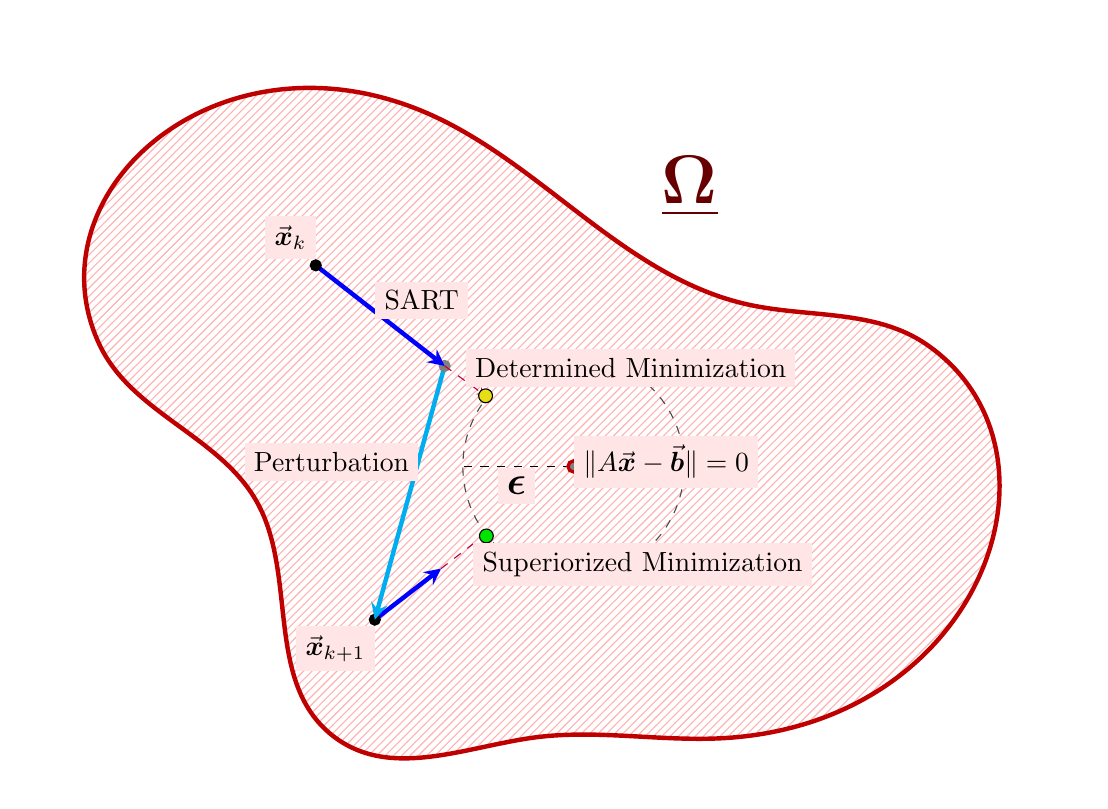
\begin{tikzpicture}
        %%BLOB
        % Fill texture
        \path[fill, pattern=north east lines, pattern color=red!30, use Hobby shortcut, closed=true] (-0.5,0.5) .. (-1.5,3.5) .. (-3.5,5.5) .. (0.5,8.5) .. (4.75,6)        .. (7,5.5) .. (4.5,0.5) .. (2,0.5);
        
        % Outline
        \path[draw, color=red!75!black, use Hobby shortcut,style=ultra thick,  closed=true] (-0.5,0.5) .. (-1.5,3.5) .. (-3.5,5.5) .. (0.5,8.5) .. (4.75,6) ..  (7,5.5) .. (4.5,0.5) .. (2,0.5) ;
        
        
        %%FEATURES
        %x_{k+2}
        %\filldraw[gray] (0.8412303782580688, 2.648688736716894) circle (2pt);
        
        % New approach continuation
        \path[draw,color=purple,-stealth,style=dashed,use Hobby shortcut,closed=false] (0.8412303782580688, 2.648688736716894) .. (1.456845567387103, 3.12303310507534);
        
        % New approach
        \path[draw,color=blue,-stealth,style=ultra thick,use Hobby shortcut,closed=false] (0, 2) .. (0.8412303782580688, 2.648688736716894);
        
        %x_{k+1\phi} /  x_{k+1}
        %\filldraw[gray] (0,2) circle (2pt);
        \filldraw[black] (0,2) circle (2pt);
        
        % Perturbation
        \path[draw,color=cyan,-stealth,style=ultra thick,use Hobby shortcut,closed=false] (0.886845567387103, 5.22303310507534) .. (0,2);
        
        %x_{k+1} / k-intermediate
        \filldraw[gray] (0.8868455673871032, 5.223033105075341) circle (2pt);
        
        % Initial approach continuation
        \path[draw,color=purple,-stealth,style=dashed,use Hobby shortcut,closed=false] (0.8868455673871032, 5.223033105075341) .. (1.406845567387103, 4.84303310507534);
        
        % Initial approach
        \path[draw,color=blue,-stealth,style=ultra thick,use Hobby shortcut,closed=false] (-0.75, 6.5) .. (0.8868455673871032, 5.223033105075341);
        
        % x_k
        \filldraw [black] (-0.75, 6.5) circle (2pt);
        
        % Epsilon radius
        \draw [style=dashed,black] (2.5, 3.95) -- (1.1,3.95);
        
        % Exact solution
        \filldraw [color=red!75!black,fill=gray,very thick] (2.5236911347742064, 3.9460662101506827) circle (2pt);
        
        % Epsilon circle
        \draw[color=gray!60!black,style=dashed] (2.5236911347742064, 3.9460662101506827) circle (40pt);
        
        % Non-superiorized solution
        \filldraw [color=black,fill=yellow!90!black] (1.406845567387103, 4.84303310507534) circle (2.5pt);
        
        % Superiorized solution
        \filldraw [color=black,fill=green!90!black] (1.416845567387103, 3.06303310507534) circle (2.5pt);
        
        
        %%LABELS
        \node[red!40!black] (c) at (4,7.5) {\Huge\textbf{\underline{$\boldsymbol{\Omega}$}}};
        %\node[fill=red!10!] (c) at (-1.8,6.8) {Starting Point};
        \node[fill=red!10!] (c) at (-1.07,6.85) {$\vvec{x}_k$};
        %\node[fill=red!10!] (c) at (1.92,6.1) {SART convergence vector};
        \node[fill=red!10!] (c) at (0.595,6.056) {SART};
        %\node[fill=red!10!] (c) at (1.4, 5.6) {$\vvec{x}_{k+1}$};
        \node[fill=red!10!] (c) at (3.25,5.2) {Determined Minimization};
        %\node[fill=red!10!] (c) at (3.35,5.2) {Non-Superiorized solution};
        %\node[fill=red!10!] (c) at (0.2,4.1) {$\phi$};
        \node[fill=red!10!] (c) at (-0.55,4) {Perturbation};
        %\node[fill=red!10!] (c) at (0.58,1.6) {$\vvec{x}_{(k+1)\phi}$};
        \node[fill=red!10!] (c) at (-0.5,1.63) {$\vvec{x}_{k+1}$};
        \node[fill=red!10!] (c) at (1.8,3.7) {\Large$\boldsymbol{\eps}$};
        %\node[fill=red!10!] (c) at (1.9,4.2) {\Large$\boldsymbol{\eps}$};
        \node[fill=red!10!] (c) at (3.4,2.7) {Superiorized Minimization};
        %\node[fill=red!10!] (c) at (2.65,1.95) {Superiorized convergence vector};
        %\node[fill=red!10!] (c) at (1,1.95) {SART$_\phi$};
        %\node[fill=red!10!] (c) at (1.4, 2.31) {$\vvec{x}_{k+2}$};
        %\node[fill=red!10!] (c) at (3.7,4.005) {Exact Solution};
        \node[fill=red!10!] (c) at (3.7,4.005) {$\norm{A\vvec{x}-\vvec{b}}=0$};
          
    \end{tikzpicture}
    \end{adjustbox}
    \caption{Simplified depiction of the way in which superiorization can guide SART towards a more optimal solution.}
    \label{blob}
\end{figure}

Then, as iterative applications of a procedure in this form will effectively apply a power sequence on $T$, we know that SART will converge if and only if the spectral radius $\rho(T)<1$\cite{young1981rate}. And as SART \textit{is} guaranteed to converge\cite{jiang2003convergence}, we know, in fact, that $\rho(T)<1$.

Yet, we might still have a relatively large spectral radius such as $\rho=0.9998\ldots$ If this is the case, SART will require an extremely large number of iterations in order to converge, as an iterative algorithm of this form has a convergence rate inversely proportional to the size of $\rho$. However, with the block iterative method, $\forall i \in [1,n]$, we know that $\rho(T_i)\leq\rho(T)$, and thus that their combined product will induce a convergence factor on the order of $\rho(T)^n$. This means we can apply multiple factors of the convergence ratio during a single iteration, for the same computational cost as in the original formulation of SART, by instead forming it as\cite{hudson1994accelerated}:

\tighten
\begin{align}
    R(\vvec{x}) &= \encl{\Prod{i=1}{n}T_i}\vvec{x} + \vvec{c}
\end{align}

SART is a deterministic function. However, we know there exist infinitely many possible solutions for $\vvec{x}$ in our problem space $\Omega$ that will minimize the proximity function $\norm{A\vvec{x}-\vvec{b}}$. Knowing where in the problem space the most-ideal reconstruction is located, and how to get there from an initial approximation, is a problem left unsolved by the standard SART algorithm.

\subsection{Superiorization}\tighten
Superiorization\cite{herman2012superiorization} is a technique capable of addressing this problem. Every iteration of SART, we can alter, or ‘perturb,’ our result by utilizing a secondary function $\phi$ to emphasize any other optimality metric we desire. While SART is deterministic, we can alter its vector of approach so it will converge upon a 'superior' solution according to the quality measured by our secondary function $\phi$, as depicted in \fig{blob}.
 
Regardless of optimality metric $\phi$, a superiorized application of SART is capable of reaching any data fidelity target for $\norm{A\vvec{x}-\vvec{b}}$ attainable by a standard application of SART. In order to guarantee this convergence characteristic, the sequence of perturbations themselves must converge to zero, and be summable. To achieve this, the norm of the initial perturbation is capped at some initial value $\alpha$, and successive perturbations are reduced by a factor of some $\beta\in(0,1)$. If we take $\vvec{x}_{k+1}=R(\vvec{x}_k)$ to be our SART procedure, the superiorized SART algorithm can be described as\cite{humphries2020comparison}:

\tighten\tighten
\begin{align}
    \vvec{x}_{k+1} &= R(\vvec{x}_k+\alpha\beta^{k-1}\vvec{v}_k)
\end{align}

Where $\vvec{v}_k=-\ds\frac{\nabla\phi(\vvec{x}_k)}{\norm{\nabla\phi(\vvec{x}_k)}}$, the unit vector in the direction of gradient descent for our secondary optimality metric $\phi$.

As our aim is to reduce noise, one obvious choice for $\phi$ would be the total variation (TV) function. The TV function is a measurement of variation between adjacent pixels in an image, and is calculated by forming the sum of something like the 'euclidean distance' in the saturation of each pixel, with two of its adjacent pixels\cite{pnp}:

\tighten
\begin{align}
    {TV}(\vvec{x}) &= \Sum{m,n}{}\sqrt{\enc{\vvec{x}_{m+1,n} - \vvec{x}_{m,n}}^2 + \enc{\vvec{x}_{m,n+1} - \vvec{x}_{m,n}}^2 + \eps^2}
\end{align}

This approach reduces noise, but also introduces a blotchy, over-smoothed quality to the image that can obscure small features. As medical imaging is often used to detect small features (fractures, the beginnings of tumors, etc.), this is not optimal for our purposes. As an alternative, we experiment with utilizing the 3D Block-Matching algorithm (BM3D)\cite{dabov2007image}.

\subsection{3D Block-Matching}\tighten
The BM3D algorithm is an image denoising procedure. It works by searching a given image for similar-looking square subsets of the image (blocks), and then utilizing a 3D-transform through a stack of these blocks to further minimize variation across the already similar-looking blocks\emd assumed, then, to be noise. It can achieve some stunning results in high-definition photo restoration, and through some clever tricks, the complexity of this algorithm has been reduced to $\bigo{n}$, so it is a strong candidate for use in an iterative application such as superiorization. However, BM3D is not a differentiable function with a gradient\emd it is a denoising procedure\emd so a different approach than gradient descent must be used to generate perturbations.

\begin{figure}[b]
    \centering
    \reflectbox{\includegraphics[width=0.49\linewidth,angle=-90,origin=c]{imgs/00000001_img.png}}
    \includegraphics[width=0.49\linewidth]{imgs/lowdose_recon__2sup.png}
    \caption{Reference image, and BM3D-Superiorized reconstruction using $\boldsymbol{\sigma=10}$.}
    \label{spooky}
\end{figure}

\subsection{Plug-and-Play Superiorization}\tighten
The technique developed as an alternative to the gradient descent strategy is to set the initial perturbation equal to the normalized difference between $\vvec{x}_k$ and $\phi(\vvec{x}_k)$. We then multiply this by our $\alpha\beta^{k-1}$ as before, and that is the perturbation applied to $\vvec{x}_k$ before it is sent back to SART to generate $\vvec{x}_{k+1}$. Because a single line of code can be altered in such an algorithm to utilize any optimality algorithm desired (simply alter the function call when calculating $\phi(\vvec{x}_k)$), this approach has been coined 'plug-and-play superiorization.' \cite{pnp} 

Our initial tests to get the experiment up-and-running led to some heavy hyperparameter tuning, and a few slight modifications to the plug-and-play approach. 

\medskip
\section{Modifications}\tighten
\subsection{Initial Hyperparameter Tuning}\tighten
Our goal was to utilize BM3D as our secondary objective function $\phi$. BM3D requires one hyperparameter, $\sigma$, an estimation of the standard deviation of the noise in the image. Previous research\cite{sheng2014denoised} indicated that $\sigma = 10$ or $\sigma = 20$ may be ideal for medical imaging applications of BM3D, as a higher $\sigma$ led to smearing of finer definition. However, when we utilized this $\sigma$ value in our superiorization structure, it led to the construction of some bizarre images that, while striking, are not usable in the context of medical imaging technology. An example of this phenomenon is displayed in \fig{spooky}. After experimenting with $\sigma$ values on the integer range $[1,20]$, we discovered that even a value of $\sigma=1$ was too high. Splitting the range $(0,1)$ by steps of $0.001$, we subjectively chose $\sigma=0.02$ as a good value to proceed with for our general experiments.

At the end of each iteration of the algorithm, our proximity function $\norm{A\vvec{x}-\vvec{b}}$ is checked against some value $\eps$. If $\norm{A\vvec{x}-\vvec{b}}\leq\eps$, then we consider our method to have converged. As we are comparing this method to the general SART algorithm, we decided to first reconstruct our images using a standard SART application, running it for a fixed number of iterations. Afterwards, we read the true $\norm{A\vvec{x}-\vvec{b}}$ for each of these reconstructions, and set those as individualized $\eps$-targets for the given image at the given exposure level. This approach was chosen because the quality of any given reconstruction is highly subject-dependent, so generalized $\eps$-targets may not have served us very well globally. Further, as these targets are taken from a successful application of SART, we know that we do not run the risk of setting an unattainable target fidelity for our superiorized algorithms.

\subsection{Algorithmic Alterations}\tighten
An issue we ran into early on was that it seemed BM3D was not doing much of anything. After a period of some discovery, we learned that our initial cap on perturbations $\alpha$ was entirely too small. The norm of our initial perturbations was typically over 60, while we were utilizing an $\alpha=0.97$. This led to the first algorithmic modification to the plug-and-play structure: Instead of hyperparameterizing $\alpha$, we set our initial $\alpha = \norm{\vvec{x}-\phi(\vvec{x}_1)}$. This means the very first perturbation per reconstruction is not normalized, as before. However, to maintain summability, $\alpha$ is multiplied in successive iterations by a hyperparameter $\gamma\in(0,1)$. The behavior of $\gamma$ and its reaction to fine-tuning is different enough from the original behavior of $\beta$ to be distinguished with a different symbol.

The next big hurdle we came across was that the algorithm was taking an exceedingly large number of iterations to converge, with no subjective improvement in overall quality by the final iteration. We investigated intermediate iteration renders, and found that the superiorization step was inducing huge perturbations at early iterations, effectively erasing all progress made by SART in the previous step. These perturbations were eventually dampened by $\gamma$, so the algorithm still converged. However, by the end, our $\phi$ was so strongly suppressed that it did nothing to prevent SART from re-introducing fine-grained noise during the final iterations of the algorithm. 

As SART realizes broad features first, the fine-grained systemic noise from our measurements doesn't begin to appear in our intermediate reconstructions until after the first handful of iterations, so inducing perturbations early on achieves little more than blurring the image, preventing those broad features from coalescing until $\phi$ is sufficiently suppressed by $\gamma$. And with the full magnitude of initial perturbation being utilized, SART requires a few iterations to pull itself back on track once we've nudged it in the direction we want.

So our solution to the problem was to modify when in the convergence cycle $\phi$ would be invoked. We landed upon a two-pronged approach. First, wait a certain number of SART iterations before the first superiorization step occurs (set by hyperparameter $k$min). And second, only perform the superiorization step every few iterations (set by hyperparameter $k$step). There is a $k$max hyperparameter as well, but we set this arbitrarily large for our experiments to ensure each algorithm would have the chance to fully express itself. Then, for any given image reconstruction, our plug-and-play+ superiorization algorithm reads as in $\enc{\textit{alg.}\ref{fig:alg}}$.


\medskip
\section{Experimental Methodology}\tighten
Our experiments began by selecting a set of 20 real-world CT image reconstructions at $512\times512$ resolution. We then took these images and reverse-transformed them back into sinograms by re-measuring them with fanbeam projections constructed using the Astra toolbox\cite{palenstijn2011performance} for Python. We created reconstructions for each sinogram at three different exposure levels, introducing Poisson noise proportional to the simulated count rate. The three different exposure levels used were:

\begin{itemize}
    \item $1\e{4}$
    \item $2.5\e{4}$
    \item $5\e{4}$
\end{itemize}

We then reconstructed approximations of the original reconstructions $\vvec{x}_{\text{ref}}$ by passing these noisy sinograms through four different variations on the algorithms described above:

\begin{itemize}
    \item SART
    \item BM3D-superiorized plug-and-play+ SART
    \item TV-superiorized SART
    \item SART with BM3D post-processing (single application)
\end{itemize}

Each resultant reconstruction was then compared to its reference image. For each combination of reconstruction technique and exposure level, the mean across the entire image set of four different metrics are taken. The four metrics included in our analysis are:

\begin{itemize}
    \item PSNR \hspace*{55pt}(peak signal-to-noise ratio)
    \item SSIM\cite{wang2004image} \hspace*{42pt}(structural similarity index)
    \item $\Delta$TV \hspace*{58pt}$\enc{TV\enc{\vvec{x}} - TV\enc{\vvec{x}_{\text{ref}}}}$
    \item Time to Converge \hspace*{13pt}(iterations to converge, times $n$subsets)
\end{itemize}

Since the number of subsets utilized is inversely proportional to the number of iterations required to converge, if we wish to effectively measure and compare convergence rates of these algorithms, $n$ needs to be taken into account. We have done so by multiplying $n$ into the number of iterations to converge, including for the fixed-number of iterations used to generate the $\eps$-targets as discussed in the previous section. We tuned the rest of our hyperparameters to $\gamma=0.75$, $\sigma=0.02$, and the variable hyperparameters displayed in \fig{params}. The entire suite of command line literals used to generate the data for our experiment is displayed in \fig{literals}.

\begin{algorithm}[t]
\caption{Plug-and-Play+ Superiorization Algorithm.}
    \label{fig:alg}
\For{$k \in[1,kmax]$}{
    \If{$(k\geq kmin) \wedge ((k-kmin)\bmod(kstep) = 0)$}{
        $x_{\phi} \gets \phi(x)$ \tcp*[r]{BM3D}
        $perturb \gets (x-x_{\phi});$ \\
        $pnorm \gets \norm{perturb}_{fro};$ \\
        \eIf{$k=kmin$}{
            $\alpha \gets pnorm;$
        }{$\alpha \gets \alpha\times\gamma;$}
        \eIf{$pnorm > \alpha$}{
            $perturb \gets \frac{\alpha \times perturb}{pnorm};$ \\ $x\gets x+p;$}
            {$x \gets x_{\phi}$;}
    }
    $x \gets R(x)$ \tcp*[r]{SART} 
    \If{$\norm{Ax-b}_{\text{fro}}\leq\eps$}{export image;\\break;}}
\end{algorithm}

\begin{figure}[h]
\caption{Variable Hyperparameters for Test Set Generation}
\label{params}
\begin{adjustbox}{width=\linewidth}
\begin{tabular}[c]{|c||c|c|c|c|}
    \hline
    {Exposure}  &{$k$min}  &{$k$step}  &{Mean $\eps$-Target} &{Conv. Time to Gen. $\eps$} \\
    \hline\hline
    $~~1\e{4}$  &~5  &4  &41.869  &144  \\\hline
    $2.5\e{4}~$ &10  &5  &26.040  &216 \\\hline
    $~~5\e{4}$  &15  &5  &16.170  &324 \\\hline
\end{tabular}
\end{adjustbox}
\end{figure}

\medskip
\section{Results}\tighten
A more in-depth table with thumbnails of each of our 20 reference images, and the individual $\eps$-targets set for each of them at each exposure level, can be found in the table in \fig{epsfull}. Also included is the mean $\eps$-target across the three exposure levels for each individual image. As the $\eps$-targets were generated from a fixed convergence time, this illustrates the principle that imaging denser material with CT results in less accurate results\emd as we see that the images of bonier areas have higher, and thus noisier, mean $\eps$-targets.

In \fig{graphs}, we show the results of our metrics analysis in both table and bar graph form. The first graph shows that the single, post-processing application of BM3D does little to improve the PSNR score over the standard SART algorithm alone. Both of our superiorized algorithms perform somewhat better than the standard SART procedure, and it does seem that the BM3D version pulls ahead of the TV one at the higher exposure level, but it is unclear from this data whether BM3D outperforms TV overall in terms of PSNR.

The SSIM scores are extremely close, and are even closer than they may at first appear, as the $y$-axis is on the range $[0.9,1]$. Perhaps not surprisingly (as BM3D was developed explicitly with SSIM in mind), the single-application of BM3D as a SART post-processing step seems to do the most in improving this score. Again, it is somewhat unclear from this data which of our superiorized algorithms outperforms the other. There is only $\sim\hspace*{-2pt}0.8\%$ difference in their performance at the $5\e{4}$ exposure level, which does not show significance. Yet, it does seem they are each reliably somewhat better than the standard SART algorithm in terms of SSIM score.

While the PSNR and SSIM metrics do not seem to deliver definitive results, there is one category with a clear outlier: TV-superiorization underperforms in terms of convergence time compared to the other algorithms by a factor of over $400\%$ at the $5\e{4}$ level. It should be noted that we have not taken into account the cost of evaluating BM3D itself versus evaluation of the gradient descent of the TV function in our calculations for convergence time. Nor do we track the difference in number of evaluations of each of these functions due to the introduction of the $k$min and $k$step hyperparameters. If considered, there may be found an even more extreme difference than what is calculated here, as we know BM3D is not performed every iteration, and that it is of order $\bigo{n}$. However, this data does illuminate a possible cause for some of the aggressive over-smoothing often induced by TV-superiorization, as the perturbations in this method are applied much more numerously than with the plug-and-play+ approach.

We also see that TV-superiorization may not even outperform the others in terms of $\Delta$TV. Notice that this graph has both positive and negative values, with negative values representing a reduction in TV compared to the original image. It may be more useful to look at magnitudes for this metric, as we \textit{should} want to roughly \textit{match} the TV of the true image. But in terms of TV \textit{reduction}, we see the BM3D post-processing procedure goes far beyond what the other algorithms are doing, especially at the $5\e{4}$ exposure level. This does seem to correspond to the way BM3D post-processed images look blurrier (albeit less noisy) than the others. Surprisingly, the standard SART algorithm seems to most closely match the TV of the reference image at the two lowest exposure levels, which may indicate that TV-superiorization is doing too much in early iterations\emd further suggesting that its aggressive oversmoothing might be tamed by utilizing tactics similar to that of the $k$min and $k$step hyperparameters introduced with the plug-and-play+ specification. The BM3D-superiorized algorithm also seems to perform better than the TV-superiorized algorithm during the first two exposure levels, but after flipping sign compared to the reference image, TV-superiorization is shown capable of reducing TV more handily than either of the others.

Finally, in \fig{pelvis}, \fig{liver}, and \fig{lung}, we have chosen three individual images to juxtapose for subjective comparison: cross-sections of a pelvic region, abdomen/liver, and chest/lungs, respectively. Each row of these figures contains the reference image\emd and then the SART, BM3D-superiorized, TV-superiorized, and BM3D post-processed reconstructions at a single exposure level. Immediately below the full images are subsections of each image that have been zoomed-in on, where some interesting detail can be observed for finer comparison. The first pair of rows of each figure are the $1\e{4}$ reconstructions, with the second pair being the $2.5\e{4}$ reconstructions. The $5\e{4}$ reconstructions are along the bottom.

Subjectively, the BM3D-superiorized pelvic reconstructions look the best to us, a fact that is especially clear at the lower exposure levels. As this area is extremely dense with bone, and thus noisier with inverse proportionality to the exposure level, the fact that it does even better at lower-exposure levels is impressive. Features look as they should, and while there is some contrast loss, much of the detail remains. Investigating the $1\e{4}$ row of this figure, we can also see the clearest demonstration of the qualitative differences between each algorithm: SART looks noisier, TV-superiorized looks blotchier, and the BM3D post-processed looks blurrier. The abdominal reconstructions also display these qualities, but to a lesser degree. There are many organs in this area, and the liver in particular is a fairly dense organ\emd so while there isn't as much bony material in these scans, this area of the body is still fairly dense.

With the sparse density of the chest cavity, and the finer detail of the lung, it is not as clear to us, subjectively, which is the best reconstruction method. We can definitively say that the BM3D post-processed reconstructions do not seem particularly usable in a medical context, but the other three algorithms produce images that are fairly comparable.

It is worth noticing, from the zoomed-in portions of any of these images at the $5\e{4}$ exposure level, that the cartoonish over-smoothing typically displayed by the TV-superiorized reconstruction technique is not prevalent. In tandem with TV's convergence time being so high, this may be even further suggestion that TV-superiorization might benefit from introduction of hyperparameters similar to $k$min and $k$step, as this behavior seems to align with that which we observed when first experimenting with the use of BM3D as our secondary function, before introducing those hyperparameters to the plug-and-play approach.

\medskip
\section{Further Research}\tighten
Further research might find it worthwhile to experiment more heavily with the effects of fine-tuning hyperparameters $k$min, $k$step, and $\gamma$, particularly in relation to expected density of material. Since blurriness continues being an issue, experimenting further with $\sigma$ is not out of the question either. It may also be possible that these hyperparameters will react differently to tuning for different superiorization functions $\phi$, so previously dissatisfactory optimality metrics may be worth another look under the plug-and-play+ approach. As mentioned numerous times already, our results strongly suggest that introduction of hyperparameters similar to $k$min and $k$step to the superiorization procedure for differentiable optimality functions (such as TV) may improve the performance of these algorithms, and thus warrants further research. We also notice that each algorithm seems to have its own characteristic flaws, so it may be worth experimenting with the utilization of multiple distinct optimality metrics $\phi$ within a single superiorization framework.

There is also concern about how to choose initial $\eps$-targets when the true image is unknown, as is the case in real-world applications. Too high a target, and our image won't be as clear as a standard SART application, but too low, and it will refuse to converge until it becomes as noisy as a standard SART application. Our own choices for convergence time to generate the target $\eps$ for these experiments was somewhat arbitrary, and influenced by subjective measures. It may be possible to calculate an estimate of the expected tolerances for $\norm{A\vvec{x}-\vvec{b}}$ based upon expected overall density of the area to be scanned, and the properties of the scanner itself. Another idea we had was to perform an initial full iteration of SART up to a conservatively-large fixed number, and have the target $\eps$ read from an image in this set that has been manually-selected by a technician or similar as "clear but not noisy." An extension of this idea might have a neural network trained to achieve the same goal, thus maintaining the automated nature of the system.

\begin{acks}
Special thanks to Dr. Thomas Humphries for his guidance, encouragement, and understanding over the course of this project.
\end{acks}

\bibliographystyle{ACM-Reference-Format}
\bibliography{thebib}


%—————————————————————————————————————————————————————————
\begin{figure*}[h]
\centering
\caption{Graphical and Numerical Representation of Result Metrics. \\\hspace*{-28pt}Please note: Scales of y-axes are dissimilar.}\bigskip\medskip\label{graphs}
\includegraphics[width=0.49\linewidth]{imgs/Bar Graphs/PSNR_bar.pdf}
\includegraphics[width=0.49\linewidth]{imgs/Bar Graphs/SSIM_bar.pdf} \\\bigskip
\includegraphics[width=0.49\linewidth]{imgs/Bar Graphs/TV_bar.pdf}
\includegraphics[width=0.49\linewidth]{imgs/Bar Graphs/CONV_bar.pdf} \\\bigskip\medskip
\begin{adjustbox}{width=0.98\linewidth}
\begin{tabular}[c]{|c|c||c|c|c|c|}
    \hline
    \multicolumn{6}{|c|}{\bf{Comparison of Mean Similarity Metrics Across Entire Set for Each Modified SART Algorithm}} \\
    \hline
    {Metric}  &{Exposure}  &{Standard SART}  &{~~BM3D-Superiorized~~}  &{~~TV-Superiorized~~} &{BM3D Post-Processing} \\
    \hline\hline
    \multirow[c]{3}{*}{~~~~~~~~PSNR~~~~~}  
        &$~~1\e{4}$  &33.9114  &35.2484  &35.2730  &34.0748  \\\cline{2-6}
        &$2.5\e{4}~$ &36.2556  &38.0098  &37.8916  &36.3510  \\\cline{2-6}
        &$~~5\e{4}$  &38.9779  &41.0029  &40.0803  &38.6524  \\\hline
        \hline
    \multirow[c]{3}{*}{~~~~~~~~SSIM~~~~~}
        &$~~1\e{4}$  &0.95314  &0.96694  &0.96518  &0.96139  \\\cline{2-6}
        &$2.5\e{4}~$ &0.96904  &0.97968  &0.97747  &0.97413  \\\cline{2-6}
        &$~~5\e{4}$  &0.97192  &0.98009  &0.97991  &0.98254  \\\hline
        \hline
    \multirow[c]{3}{*}{$\Delta$TV}
        &$~~1\e{4}$  &\hspace*{-5pt}+156.403  &\hspace*{-5pt}-395.548   &\hspace*{-5pt}-704.306  &\hspace*{-5pt}-843.237  \\\cline{2-6}
        &$2.5\e{4}~$ &\hspace*{-5pt}+170.532  &\hspace*{-5pt}-340.048   &\hspace*{-5pt}-642.536  &\hspace*{-5pt}-750.439  \\\cline{2-6}
        &$~~5\e{4}$  &\hspace*{-5pt}+785.614  &\hspace*{-5pt}+549.064   &\hspace*{-5pt}+199.582  &\hspace*{-5pt}-658.002  \\\hline
        \hline
    \multirow[c]{3}{*}{$~~\mathclap{\substack{\text{Time}\\\text{to}\\\text{Converge}}}$}
        &$~~1\e{4}$  &144  &126.0   &442.2  &\emd  \\\cline{2-6}
        &$2.5\e{4}~$ &216  &216.6   &852.0  &\emd  \\\cline{2-6}
        &$~~5\e{4}$  &324  &735.6   &\hspace*{-3.5pt}4041.0  &\emd  \\\hline
\end{tabular}
\end{adjustbox}
\end{figure*}
%—————————————————————————————————————————————————————————

%—————————————————————————————————————————————————————————
\begin{figure*}[h]
    \centering
    \caption{Comparison of image 3817 (pelvis) with each resultant reconstruction. Lowest exposure level first.}
    \label{pelvis}
    \begin{tabular}[c]{|c|c|c|c|c|}
        \hline
        \makebox[0.18\linewidth][c]{Reference} & \makebox[0.18\linewidth][c]{SART} & \makebox[0.18\linewidth][c]{BM3D-Superiorized} & \makebox[0.18\linewidth][c]{TV-Superiorized} & \makebox[0.18\linewidth][c]{BM3D Post} \\
        \hline
    \end{tabular}
    \begin{tikzpicture}
    \node[anchor=south west,inner sep=0] (image) at (0,0) {\includegraphics[width=\linewidth]{imgs/Comp1/14.png}};
    \begin{scope}[x={(image.south east)},y={(image.north west)}]
        \draw[red,ultra thick] (0.085546875,0.265625) rectangle (0.149609375,0.5859375);
        \path[draw,color=red,-stealth,style=dashed,use Hobby shortcut,closed=false] (0.085546875,0.265625) .. (0,0);
        \path[draw,color=red,-stealth,style=dashed,use Hobby shortcut,closed=false] (0.149609375,0.265625) .. (0.2,0);
    \end{scope}
    \end{tikzpicture} \\
    \vspace*{-2pt}
    \includegraphics[width=\linewidth]{imgs/Comp1/14_z3.png} \\
    \vspace*{-1pt}
    \includegraphics[width=\linewidth]{imgs/Comp2/14.png} \\
    \vspace*{-1pt}
    \includegraphics[width=\linewidth]{imgs/Comp2/14_z3.png} \\
    \vspace*{-1pt}
    \includegraphics[width=\linewidth]{imgs/Comp3/14.png} \\
    \vspace*{-1pt}
    \includegraphics[width=\linewidth]{imgs/Comp3/14_z3.png}
\end{figure*}
%—————————————————————————————————————————————————————————

%—————————————————————————————————————————————————————————
\begin{figure*}[h]
    \centering
    \caption{Comparison of image 3883 (liver) with each resultant reconstruction. Lowest exposure level first.}
    \label{liver}
    \begin{tabular}[c]{|c|c|c|c|c|}
        \hline
        \makebox[0.18\linewidth][c]{Reference} & \makebox[0.18\linewidth][c]{SART} & \makebox[0.18\linewidth][c]{BM3D-Superiorized} & \makebox[0.18\linewidth][c]{TV-Superiorized} & \makebox[0.18\linewidth][c]{BM3D Post} \\
        \hline
    \end{tabular}
    \begin{tikzpicture}
    \node[anchor=south west,inner sep=0] (image) at (0,0) {\includegraphics[width=\linewidth]{imgs/Comp1/15.png}};
    \begin{scope}[x={(image.south east)},y={(image.north west)}]
        \draw[red,ultra thick] (0.10625,0.271484375) rectangle (0.16875,0.583984375);
        \path[draw,color=red,-stealth,style=dashed,use Hobby shortcut,closed=false] (0.10625,0.271484375) .. (0,0);
        \path[draw,color=red,-stealth,style=dashed,use Hobby shortcut,closed=false] (0.16875,0.271484375) .. (0.2,0);
    \end{scope}
    \end{tikzpicture} \\
    \vspace*{-2pt}
    \includegraphics[width=\linewidth]{imgs/Comp1/15_z1.png} \\
    \vspace*{-1pt}
    \includegraphics[width=\linewidth]{imgs/Comp2/15.png} \\
    \vspace*{-1pt}
    \includegraphics[width=\linewidth]{imgs/Comp2/15_z1.png} \\
    \vspace*{-1pt}
    \includegraphics[width=\linewidth]{imgs/Comp3/15.png} \\
    \vspace*{-1pt}
    \includegraphics[width=\linewidth]{imgs/Comp3/15_z1.png}
\end{figure*}
%—————————————————————————————————————————————————————————

%—————————————————————————————————————————————————————————
\begin{figure*}[h]
    \centering
    \caption{Comparison of image 3803 (lung) with each resultant reconstruction. Lowest exposure level first.}
    \label{lung}
    \begin{tabular}[c]{|c|c|c|c|c|}
        \hline
        \makebox[0.18\linewidth][c]{Reference} & \makebox[0.18\linewidth][c]{SART} & \makebox[0.18\linewidth][c]{BM3D-Superiorized} & \makebox[0.18\linewidth][c]{TV-Superiorized} & \makebox[0.18\linewidth][c]{BM3D Post} \\
        \hline
    \end{tabular}
    \begin{tikzpicture}
    \node[anchor=south west,inner sep=0] (image) at (0,0) {\includegraphics[width=\linewidth]{imgs/Comp1/12.png}};
    \begin{scope}[x={(image.south east)},y={(image.north west)}]
        \draw[red,ultra thick] (0.03828125,0.1484375) rectangle (0.091015625,0.3984375);
        \path[draw,color=red,-stealth,style=dashed,use Hobby shortcut,closed=false] (0.03828125,0.1484375) .. (0,0);
        \path[draw,color=red,-stealth,style=dashed,use Hobby shortcut,closed=false] (0.091015625,0.1484375) .. (0.2,0);
    \end{scope}
    \end{tikzpicture} \\
    \vspace*{-2pt}
    \includegraphics[width=\linewidth]{imgs/Comp1/12_z2.png} \\
    \vspace*{-1pt}
    \includegraphics[width=\linewidth]{imgs/Comp2/12.png} \\
    \vspace*{-1pt}
    \includegraphics[width=\linewidth]{imgs/Comp2/12_z2.png} \\
    \vspace*{-1pt}
    \includegraphics[width=\linewidth]{imgs/Comp3/12.png} \\
    \vspace*{-1pt}
    \includegraphics[width=\linewidth]{imgs/Comp3/12_z2.png}
\end{figure*}
%—————————————————————————————————————————————————————————

%—————————————————————————————————————————————————————————
\begin{figure*}[h]
    \centering
    \caption{\Large$\eps$\normalsize-Targets for individual images at each exposure level.}
    \label{epsfull}
    \begin{adjustbox}{width=\linewidth}
    \begin{tabular}[c]{|c||c|c|c|c|||c||c|c|c|c|}
        \hline
        {Image}  &{$1\e{4}$}  &{$2.5\e{4}$}  &{$5\e{4}$}  &{Mean (img)}  &{Image}  &{$1\e{4}$}  &{$2.5\e{4}$}  &{$5\e{4}$} &{Mean (img)} \\
        \hline\hline
        3629 &  &  &  &  &3792 &  &  &  &  \\        
        \reflectbox{\includegraphics[width=0.05\textheight,angle=-90,origin=c]{imgs/Test Set/00003629_img.png}}  &33.798305  &21.034120  &12.507258  &22.446561  &\reflectbox{\includegraphics[width=0.05\textheight,angle=-90,origin=c]{imgs/Test Set/00003792_img.png}}  &49.304163  &30.389597  &19.694704  &33.129488  \\\hline
        3645&&&&&3803&&&&\\
        \reflectbox{\includegraphics[width=0.05\textheight,angle=-90,origin=c]{imgs/Test Set/00003645_img.png}}  &37.816196  &23.376304  &14.643529  &25.278676  &\reflectbox{\includegraphics[width=0.05\textheight,angle=-90,origin=c]{imgs/Test Set/00003803_img.png}}  &40.873823  &25.612410  &15.892331  &27.459521  \\\hline
        3665&&&&&3816&&&&\\
        \reflectbox{\includegraphics[width=0.05\textheight,angle=-90,origin=c]{imgs/Test Set/00003665_img.png}}  &36.010247  &22.460129  &13.554755  &24.008377  &\reflectbox{\includegraphics[width=0.05\textheight,angle=-90,origin=c]{imgs/Test Set/00003816_img.png}}  &36.329424  &22.630560  &13.878041  &24.279341  \\\hline
        3689&&&&&3817&&&&\\
        \reflectbox{\includegraphics[width=0.05\textheight,angle=-90,origin=c]{imgs/Test Set/00003689_img.png}}  &55.240813  &34.216626  &21.513963  &36.990467  &\reflectbox{\includegraphics[width=0.05\textheight,angle=-90,origin=c]{imgs/Test Set/00003817_img.png}}  &47.173994  &29.035184  &18.776478  &31.661885  \\\hline
        3696&&&&&3845&&&&\\
        \reflectbox{\includegraphics[width=0.05\textheight,angle=-90,origin=c]{imgs/Test Set/00003696_img.png}}  &40.633332  &25.548050  &15.330123  &27.170501  &\reflectbox{\includegraphics[width=0.05\textheight,angle=-90,origin=c]{imgs/Test Set/00003845_img.png}}  &32.889000  &20.913214  &12.570747  &22.124320  \\\hline
        3705&&&&&3883&&&&\\
        \reflectbox{\includegraphics[width=0.05\textheight,angle=-90,origin=c]{imgs/Test Set/00003705_img.png}}  &40.798881  &25.625331  &15.199934  &27.208048  &\reflectbox{\includegraphics[width=0.05\textheight,angle=-90,origin=c]{imgs/Test Set/00003883_img.png}}  &44.649725  &27.431934  &17.188574  &29.756744  \\\hline
        3716&&&&&3895&&&&\\
        \reflectbox{\includegraphics[width=0.05\textheight,angle=-90,origin=c]{imgs/Test Set/00003716_img.png}}  &40.734763  &25.687267  &15.374747  &27.265592  &\reflectbox{\includegraphics[width=0.05\textheight,angle=-90,origin=c]{imgs/Test Set/00003895_img.png}}  &55.245939  &34.078170  &22.485325  &37.269811  \\\hline
        3743&&&&&3924&&&&\\
        \reflectbox{\includegraphics[width=0.05\textheight,angle=-90,origin=c]{imgs/Test Set/00003743_img.png}}  &40.442785  &25.538445  &14.986390  &26.989206  &\reflectbox{\includegraphics[width=0.05\textheight,angle=-90,origin=c]{imgs/Test Set/00003924_img.png}}  &30.201796  &18.853552  &11.022670  &20.026006  \\\hline
        3782&&&&&3932&&&&\\
        \reflectbox{\includegraphics[width=0.05\textheight,angle=-90,origin=c]{imgs/Test Set/00003782_img.png}}  &37.717053  &23.428681  &14.476626  &25.207453  &\reflectbox{\includegraphics[width=0.05\textheight,angle=-90,origin=c]{imgs/Test Set/00003932_img.png}}  &51.042544  &31.393727  &20.456598  &34.297623  \\\hline
        3784&&&&&3952&&&&\\
        \reflectbox{\includegraphics[width=0.05\textheight,angle=-90,origin=c]{imgs/Test Set/00003784_img.png}}  &40.918422  &25.368276  &15.900568  &27.395755  &\reflectbox{\includegraphics[width=0.05\textheight,angle=-90,origin=c]{imgs/Test Set/00003952_img.png}}  &45.559636  &28.183549  &17.954075  &30.565753  \\\hline\hline
        \multicolumn{5}{r|}{}  &{Mean (set)}  &41.869     &26.040     &16.170     &28.026333  \\\cline{6-10}
    \end{tabular}
    \end{adjustbox}
    \label{fig:eps}
\end{figure*}
%—————————————————————————————————————————————————————————

%—————————————————————————————————————————————————————————
\begin{figure*}[h]
\Huge\caption{Command line arguments used for batch generation of files.}\label{literals}\bigskip
\large\begin{center}\underline{SINOGRAMS}\end{center}\smallskip\normalsize
\begin{verbatim}
python make_sino.py --in /data/CT_data/bm3d_test_set/ --out sinos/1e4 --psize 0.0568 --range 0 360
                    --counts 1e4
\end{verbatim}\smallskip
\begin{verbatim}
python make_sino.py --in /data/CT_data/bm3d_test_set/ --out sinos/2.5e4 --psize 0.0568 --range 0 360
                    --counts 2.5e4
\end{verbatim}\smallskip
\begin{verbatim}
python make_sino.py --in /data/CT_data/bm3d_test_set/ --out sinos/5e4 --psize 0.0568 --range 0 360
                    --counts 5e4
\end{verbatim}\bigskip

\large\begin{center}\underline{SART \& \huge$\eps$\large-TARGETS}\end{center}\smallskip\normalsize
\begin{verbatim}
python SART_pnp_BM3D_new.py --sino sinos/1e4 --out recons/1e4 --psize 0.0568 --range 0 360 --nsubs 18 
                            --numits 8 --make_png True
\end{verbatim}\smallskip
\begin{verbatim}
python SART_pnp_BM3D_new.py --sino sinos/2.5e4 --out recons/2.5e4 --psize 0.0568 --range 0 360 --nsubs 18 
                            --numits 12 --make_png True
\end{verbatim}\smallskip
\begin{verbatim}
python SART_pnp_BM3D_new.py --sino sinos/5e4 --out  recons/5e4 --psize 0.0568 --range 0 360 --nsubs 18 
                            --numits 18 --make_png True
\end{verbatim}\bigskip

\large\begin{center}\underline{BM3D SUPERIORIZED}\end{center}\smallskip\normalsize
\begin{verbatim}
python SART_pnp_BM3D_new.py --sino sinos/1e4 --out recons/1e4 --psize 0.0568 --range 0 360 --nsubs 12
                            --numits 10000000000 --make_png True --sup_params 5 4 0.75 0.02
                            --epsilon_target recons/1e4/t_residuals.txt
\end{verbatim}\smallskip
\begin{verbatim}
python SART_pnp_BM3D_new.py --sino sinos/2.5e4 --out recons/2.5e4 --psize 0.0568 --range 0 360 --nsubs 12
                            --numits 10000000000 --make_png True --sup_params 10 5 0.75 0.02
                            --epsilon_target recons/2.5e4/t_residuals.txt
\end{verbatim}\smallskip
\begin{verbatim}
python SART_pnp_BM3D_new.py --sino sinos/5e4 --out recons/5e4 --psize 0.0568 --range 0 360 --nsubs 12
                            --numits 10000000000 --make_png True --sup_params 15 5 0.75 0.02
                            --epsilon_target recons/5e4/t_residuals.txt
\end{verbatim}\bigskip

\large\begin{center}\underline{TV SUPERIORIZED}\end{center}\smallskip\normalsize
\begin{verbatim}
python SART.py --sino recons/1e4/2_SINO --out recons/1e4/6_TVsup --psize 0.0568 --range 0 360 --nsubs 12
               --numits 10000000000 --sup_params 0.9995 20 0.5 --epsilon_target recons/1e4/t_residuals.txt
\end{verbatim}\smallskip
\begin{verbatim}
python SART.py --sino recons/2.5e4/2_SINO --out recons/2.5e4/6_TVsup --psize 0.0568 --range 0 360 --nsubs 12 
               --numits 10000000000 --sup_params 0.9995 20 0.5 --epsilon_target recons/2.5e4/t_residuals.txt
\end{verbatim}\smallskip
\begin{verbatim}
python SART.py --sino recons/5e4/2_SINO --out recons/5e4/6_TVsup --psize 0.0568 --range 0 360 --nsubs 12 
               --numits 10000000000 --sup_params 0.9995 20 0.5 --epsilon_target recons/5e4/t_residuals.txt
\end{verbatim}\bigskip

\large\begin{center}\underline{BM3D POST-PROCESSED}\end{center}\smallskip\normalsize
\begin{verbatim}
python SART_pnp_BM3D_new.py --sino sinos/1e4 --out recons --psize 0.0568 --range 0 360 --nsubs 12 --numits 9 
                            --make_png True --make_intermediate True --sup_params 9 5 0.75 0.02
\end{verbatim}\smallskip
\begin{verbatim}
python SART_pnp_BM3D_new.py --sino sinos/2.5e4 --out recons --psize 0.0568 --range 0 360 --nsubs 12 --numits 13 
                            --make_png True --make_intermediate True --sup_params 13 5 0.75 0.02
\end{verbatim}\smallskip
\begin{verbatim}
python SART_pnp_BM3D_new.py --sino sinos/5e4 --out recons --psize 0.0568 --range 0 360 --nsubs 12 --numits 16 
                            --make_png True --make_intermediate True --sup_params 19 5 0.75 0.02
\end{verbatim}
\end{figure*}
%—————————————————————————————————————————————————————————




\end{document}